\documentclass[12pt]{article}

\usepackage[hidelinks]{hyperref}    
\usepackage[all]{hypcap}
\usepackage{amssymb}
\usepackage{amsmath}
\usepackage{listings}
\usepackage{xcolor}
\usepackage{graphicx}
\usepackage{float}

\definecolor{commentcolor}{rgb}{0.5, 0.5, 0.5}
\definecolor{keywordcolor}{rgb}{0, 0, 1}
\definecolor{stringcolor}{rgb}{0.58, 0, 0.82}

% C++ settings
\lstset{ 
    language=C++,
    basicstyle=\ttfamily\footnotesize,
    keywordstyle=\color{keywordcolor}\bfseries,
    commentstyle=\color{commentcolor}\itshape,
    stringstyle=\color{stringcolor},
    numbers=left,                   % Position of line numbers
    numberstyle=\tiny,              % Size of line numbers
    stepnumber=1,                   % Increment of line numbers
    numbersep=10pt,                 % Distance from line numbers to code
    backgroundcolor=\color{white},  % Background color
    showspaces=false,               % Show spaces
    showstringspaces=false,         % Show spaces in strings
    showtabs=false,                 % Show tabs
    frame=single,                   % Frame code box
    tabsize=4,                      % Tab size
    captionpos=b,                   % Position of captions
    breaklines=true,                % Line breaking
    breakatwhitespace=false,        % Break at whitespace
    escapeinside={\%*}{*)}          % Escape to LaTeX
}

\graphicspath{{./_images/}}

\title{\textbf{Programmazione}}
\date{Settembre 2024 - ..}
\author{Andrea Malvezzi}

\begin{document}

\maketitle

\pagebreak
\tableofcontents

\pagebreak
\section{HEAP e STACK}
\label{sec:HEAP_STACK}
L'HEAP e lo STACK sono due divisioni della memoria in cui vengono salvati i dati durante l'esecuzione di un programma. 
I due svolgono due ruoli diversi ma fondamentali:

\subsection{L'HEAP}
\label{ssec:HEAP}
L'HEAP è una porzione di memoria dedicata all'allocazione dinamica delle variabili, quindi mediante istruzioni come new e delete. Grazie a questa dinamicità, qui si possono sfruttare strutture dati di lunghezza indefinita, come liste o alberi, ma con una rapidità limitata.

\subsection{Lo STACK}
\label{ssec:STACK}
Lo STACK è una porzione di memoria dedicata alla gestione automatica (quindi a cura del compilatore) di variabili locali e simili. Accedere ai dati al suo interno risulta veloce grazie alla filosofia LIFO (Last-In-First-Out).

\section{Puntatori}
\label{sec:pointers}

\subsection{Cosa sono e come si definiscono}
\label{ssec:whats_pointers}
Un puntatore è uno speciale tipo di dato capace di immagazzinare un indirizzo di memoria corrispondente ad un altro dato. \\
Quando si dichiara un puntatore bisogna specificare il tipo di dato a cui lo si vuole far puntare. Vediamo un esempio pratico:
\begin{lstlisting}
    int *int_p;         // Questo punta a un intero
    char *char_p;       // Questo punta a un carattere
    // E via dicendo ...
\end{lstlisting}
Inoltre in cpp la dichiarazione di un puntatore ha una sintassi variabile: il * può difatti essere posto dopo il tipo di puntatore o prima del nome di questo. A causa di questa caratteristica bisogna tuttavia prestare attenzione a quando si vogliono dichiarare due puntatori nella stessa riga:
\begin{lstlisting}
    // Qui r corrisponde a un intero, non a un puntatore!
    int* p, r;

    // Per due puntatori, occorre usare la seguente sintassi:
    int *p, *r;
\end{lstlisting}

\subsection{Operazioni con i puntatori}
\label{ssec:pointers_operations}
Si possono effettuare operazioni diversi con i puntatori, tra cui le più importanti sono:

\subsubsection{NULL}
\label{sssec:NULL_operator}
Quando si assegna il valore NULL a un puntatore si indica che questo non punta a nessuna cella di memoria. Si usa spesso in seguito all'istruzione \hyperref[sssec:delete_operator]{delete}.
\begin{lstlisting}
    int *p = NULL;      // p non punta a una cella di memoria
\end{lstlisting}

\subsubsection{Operatore \&}
\label{sssec:ampersand_operator}
L'operatore ampersand '\&' si usa in due contesti: per ottenere l'indirizzo di una variabile e per creare un riferimento a questa.
Il primo caso risulta utile quando si vuole creare un puntatore ad una certa variabile:
\begin{lstlisting}
    int n = 10;
    int *n_p = &n;      // ora n_p punta all'indirizzo di n!
\end{lstlisting}
Mentre il secondo caso risulta più utile quando si vuole creare un alias di una variabile per modificare quest'ultima mediante reference.
\begin{lstlisting}
    int n = 10;
    int &alias_n = n;   // reference ad n
    alias_n = 20;       // n = 20;
\end{lstlisting}
La differenza sostanziale tra i due approci sta nella flessibilità: i puntatori possono essere riutilizzati e possono essere annullati, mentre le reference lavorano su una sola variabile definita esattamente alla definizione della reference stessa e non possono essere NULL.

\subsubsection{Dereferenziazione (*)}
\label{sssec:deref}
La dereferenziazione si usa in due casi: per dichiarare un puntatore e per accedere all'indirizzo a cui questo sta puntando.
\begin{lstlisting}
    int value = 42;
    int *p = &value;    // Dichiarazione puntatore
    int dereferencedValue = *p;  // Accede al valore 42
\end{lstlisting}

\subsubsection{Istruzione new}
\label{sssec:new_operator}
L'istruzione new alloca dinamicamente memoria (nell'HEAP), restituendo un puntatore all'area di memoria allocata.
\begin{lstlisting}
    int *p = new int;
    *p = 42;
\end{lstlisting}
Qui fare p = 42 darebbe errore: staremmo assegnando un int a un int*. Invece in questa maniera assegnamo al contenuto della cella di memoria a cui punta p il valore 42. 

\subsubsection{Istruzione delete}
\label{sssec:delete_operator}
L'operatore delete libera la memoria allocata dinamicamente mediante new.
\begin{lstlisting}
    int *p = new int;
    delete p;
    p = NULL;       // come mai p=NULL?
\end{lstlisting}
Nell'esempio fornito liberiamo la cella di memoria allocata dinamicamente con int *p = new int. Se lasciassimo *p senza una reference, questo diventerebbe un dangling pointer, ovvero un puntatore contenente un valore assegnato dal compilatore (randomico). Per evitarlo, annulliamo *p con p = NULL. 

\subsection{L'istruzione typedef}
\label{ssec:typedef_instruction}
L'istruzione typedef permette di definire un nuovo tipo, utilizzabile durante le dichiarazioni di nuovi dati. Questo risulta particolarmente utile quando si lavora con i puntatori in quanto permette di scrivere quanto segue:
\begin{lstlisting}
    // fuori dal main, idealmente ...
    typedef int *p_int;     // definisco tipo p_int

    // nel main, ora...
    p_int p, q;        // equivalente a int *p, *q

    // ho dichiarato due puntatori in una sola riga!
    // Questo permette di evitare confusione
\end{lstlisting}

\section{Strutture dati dinamiche}
\label{sec:strutture_dati_dinamiche}

\subsection{Le linked lists}
\label{ssec:linked_lists}
Una linked list corrisponde ad una sequenza di nodi di grandezza dinamica.
Questo significa che la lista non avrà una grandezza fissa, ma si adatterà alle necessità del programma scritto da noi (se implementata correttamente).

\subsubsection{Introduzione all'implementazione delle linked lists}
\label{sssec:linked_lists_introduction}
Per implementare una linked list occorrerà utilizzare la direttiva struct (per definire che cos'è un \textit{nodo})
e i puntatori, per puntare al nodo successivo e/o precedente (in questo caso si parlerebbe di doubly-linked-list).
Visualizzato, quanto appena spiegato equivale a qualcosa del genere:
\begin{figure}[H]
    \centering
    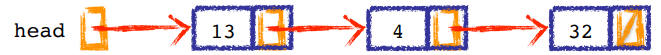
\includegraphics[width=.9\linewidth,height=.40\textheight,keepaspectratio]{linked_list_visualized.png} % essenzialmente resiza l'immagine
    \begin{center}
        \caption{\label{fig:} "Head" corrisponde ad un puntatore puntante all'indirizzo in memoria del nodo della lista. Ogni elemento (nodo) contiene inoltre un puntatore all'indirizzo del prossimo della struttura.} % label fuori da caption spesso non va, mettilo dentro
    \end{center}
\end{figure}

\subsubsection{Implementare le linked lists}
\label{sssec:linked_lists_implement}
Anzitutto, occorre capire come funziona una linked list ad un livello più profondo.
Essendo questa una struttura dati dinamica, di cui non si conosce la grandezza a priori, la si dovrà ingrandire mano a mano che si avanza nel programma.
Per farlo, occorrerà sfruttare \hyperref[sec:HEAP_STACK]{l'Heap}, mediante istruzioni come new e delete, olre che ai puntatori.
\\
Partiamo definendo la struttura dati che useremo per immagazzinare il dato da salvare e l'indirizzo del prossimo item: un \textbf{Nodo}.
\begin{lstlisting}
    struct Nodo {
        int valore;
        Nodo *next;     // Definizione circolare
    }
\end{lstlisting}
In seguito, occorrerà definire un head della lista.
Questo oggetto non corrisponderà al primo elemento della lista, ma bensì al puntatore puntante all'indirizzo del primo oggetto stesso.
Questo significa che per accedere ai campi effettivi del Nodo, occorrerà usare la dereferenziazione (*).
\begin{lstlisting}
    Nodo *head = new Nodo;   // new alloca memoria nell'Heap

    // -> corrisponde a derefernziare e usare il punto
    head -> value = 10;     // come (*head).value = 10
    head -> next = nullptr; // anche NULL andrebbe bene
\end{lstlisting}
Al termine del codice, occorre ricordarsi di liberare la memoria allocata con \textit{new}, per evitare \textbf{Memory Leaks}.
\begin{lstlisting}
    Nodo *head = new Nodo;
    ...codice...

    // al termine del codice libero la memoria allocata
    delete head;
\end{lstlisting}
Nel caso in cui si avesse una lista con molteplici elementi, occorrerebbe liberare la memoria di ognuno dei nodi di questa. Per farlo si potrebbe usare la seguente funzione:
\begin{lstlisting}
    void empty(Nodo *&head){
        // itero fino a che non ho il Nodo corrente null
        while(head != nullptr)
        {
            // creo una variabile temp per copiare head
            Nodo *temp = head;
            // sposto head al Nodo successivo
            head = head -> next;
            // cancello temp, che punta al nodo precedente
            delete temp;
        }
    }
\end{lstlisting}

\subsubsection{Operazioni sulle linked lists}
\label{sssec:linked_lists_operations}
Si possono inserire elementi all'inizio della lista, in una certa posizione, eliminare certi elementi, controllare che sia vuota $\dots$ qualunque cosa sia utile e si sia in grado di implementare.
\\
A \textcolor{blue}{\href{https://github.com/andrea-malvezzi/unibo/tree/master/ANDREA/Programmazione/Appunti/codice/Puntatori_Strutture_Dinamiche}{questo}} link è presente il codice delle operazioni più popolari inerenti alle linked lists.

\end{document}